% $Id$
% macros-paper.tex
% FIX: Switch to LaTeX2e, not 209
\documentclass[11pt]{article}
% epsfig was epsf above, and uses of \epsfig{file=dir.eps} below were
% {\epsfxsize 7in\epsfbox{dir.eps}}.
\usepackage{epsfig}

% the "fullpage" package does almost the same thing
% as the below lines-- it doesn't make things quite as
% tall or wide, but is generally what I use
% \usepackage{fullpage}
\marginparwidth 0pt
\oddsidemargin  0pt
\evensidemargin 0pt
\marginparsep 0pt

\topmargin   0pt

\textwidth   6.5 in
\textheight  8.5 in

\renewcommand{\floatpagefraction}{.8} %default .5
%\renewcommand{\textfraction}{.2}  % .2 is the default
%\renewcommand{\topfraction}{.7}   % .7 is the default

\begin{document}
% \bibliographystyle{plain}
\bibliographystyle{alpha}

\title{An Empirical Analysis of C Preprocessor Use}

\author{Michael Ernst%
  \thanks{Email addresses: \{{\tt mernst},{\tt gjb},{\tt notkin}\}{\tt @cs.washington.edu}}
  \and Greg J. Badros%
  \thanks{Supported by a National Science Foundation
    Graduate Fellowship. Any opinions, findings, conclusions, or
    recommendations expressed in this publication are those of the
    author, and do not necessarily reflect the views of the National
    Science Foundation.}
  \and David Notkin}

\date{Department of Computer
Science and Engineering\\
University of Washington\\
Box 352350\\
Seattle, WA  98195-2350  USA\\
\today}  

\maketitle

\begin{abstract}

  The C programming language is intimately connected to its macro
  preprocessor.  This relationship affects, indeed generally hinders,
  both the tools (compilers, debuggers, call graph extractors, etc.)\ 
  built to engineer C programs and also the ease of translating to other
  languages such as C++.  In this paper we analyze over 20 packages
  comprising over one million lines of publicly available C code,
  determining the ways in which the preprocessor is used in practice.
  We developed a framework for analyzing preprocessor usage and used it to
  extract information about the percentage of preprocessor directives in
  C programs, the frequency of use of defined macros, the relationship
  between C functions and their use of macros, and the macros that are
  difficult to express in terms of other C or C++ language features.  We
  report on the analysis, in particular illustrating data that are
  material when considering the development of tools for C or C++.  The
  results (and the supporting framework) lay the foundation for
  developing a tool to reduce usage of the preprocessor by translating
  from C to C++.

\end{abstract}

\bigskip

\section{Introduction}

The C programming language~\cite{ansi} is intimately connected to its macro
preprocessor, Cpp~\cite[Ch.3]{Harbison91}.  In a sense C is not a complete
programming language without the preprocessor, which supplies essential 
facilities such as
file inclusion, defining constants and macros, and conditional compilation
which are present in essentially every C program.   
While the preprocessor can be used in simple or well-structured ways to
improve portability, performance, or readability, it also lends itself to 
arbitrary source code manipulations that complicate understanding of the
program by both software engineers and tools.
This relationship
between the C language and the preprocessor has a number of consequences,
many of which were probably not anticipated by the original designers.

Stroustrup puts the consequences of this relationship in perspective:
\begin{quote}
Occasionally, even the most extreme uses of Cpp are useful, but its
facilities are so unstructured and intrusive that they are a constant
problem to programmers, maintainers, people porting code, and tool
builders~\cite[p.~424]{Stroustrup-DesignEvolution}.
\end{quote}

Tools have three options for coping with Cpp.  They may ignore preprocessor
directives (including macro definitions) altogether, accept only post-processed
code (perhaps by running Cpp on their input), or attempt to emulate the
preprocessor.

Ignoring preprocessor directives is an option for approximate tools
(such as those based on lexical or approximate parsing
techniques), but accurate information about function extents, scope
nesting, declared variables and functions, and so forth requires
addressing the preprocessor.

Operating on post-processed code, the most common strategy, is simple to
implement, but then the tool's input differs from what the
programmer sees.  Even when line number mappings are maintained, other
information is lost in the mapping back to the original source code.
For instance, source-level debuggers have no symbolic names or types
for constants introduced via {\tt \#define}.  As another example, Siff
and Reps describe a technique that uses type inferencing to produce
C++ function templates from C; however, the input is ``a C program
component that $\ldots$ has been preprocessed so that all include
files are incorporated and all macros
expanded~\cite[p.~145]{Siff-fse96}.''  Such preprocessing may limit
the readability and reusability of the resulting C++ templates.  As
yet another related example, call graph extractors generally work in
terms of the post-processed code, even when a human programmer---as
opposed to an optimizing compiler, for example---is the intended
consumer of the call graph~\cite{Murphy-icse18}.  Some tools even
leave the software engineer responsible for inferring the mapping between the
original and the post-processed source, which is an undesirable and
error-prone situation.

A tool that first preprocesses code, or insists on preprocessed code as
input, cannot be run on a non-syntactic program or one that will not
preprocess (or produces nonsense) on the platform on which the tool is being
run.  These constraints complicate porting and maintenance, two of the
situations in which program understanding and transformation tools are most
likely to be needed.  Additionally, a tool supplied with only one post-processed
instantiation of the source code cannot reason about the program as a
whole, only about that version that results from one particular set of
preprocessor variables.  (For instance, a bug in one configuration may not
be discovered despite exhaustive testing of other configurations that do
not incorporate particular code or do not admit particular paths through
the code.)

The third option, emulating the preprocessor, is fraught with difficulty.
Macro definitions consist of complete tokens but need not be complete
expressions or statements.  Conditional compilation and alternative macro
definitions lead to very different results from a single original program
text.  Preprocessing also adds complexity to an implementation.  So,
tradeoffs must be made between performing preprocessing and maintaining the
code in as close to its original form as possible.  Despite these problems,
in many situations only performing some sort of preprocessing can produce
useful answers.

All three approaches would be unnecessary if programs did not use
preprocessor directives.  This is exactly what Stroustrup suggests:
\begin{quote}
  I'd like to see Cpp abolished.  However, the only realistic and
  responsible way of doing that is first to make it redundant, then
  encourage people to use the better alternatives, and {\em then\/}---years
  later---banish Cpp into the program development environment with the
  other extra-linguistic tools where it
  belongs~\cite[p.~426]{Stroustrup-DesignEvolution}.
\end{quote}
C++ contains features---such as constant variables, inline functions,
templates, and reference parameters---that obviate many uses of Cpp.  Thus,
translation to C++
is another path for partial elimination of Cpp.  

%O'Callahan and Jackson also use type
%inference, although for program understanding rather than translation;
%they, too, apply their techniques to post-processed
%code~\cite{OCallahan-icse97}.

As a step toward such preprocessor elimination, we empirically analyzed
preprocessor usage in 24 C packages comprising just over one million lines
of code.  Figure~\ref{fig:packages} lists the packages and their sizes in
terms of physical lines (or newline characters) and non-comment, non-blank
(NCNB) lines, which disregards lines consisting of only comments or
whitespace.  The remainder of the analysis uses only the NCNB length, which
more accurately reflects the amount of source code in a package.

\begin{figure}
\centering
{\small
  \setlength{\tabcolsep}{.25em}
  \begin{tabular}{|l|r|r|}\hline
Package & Physical Lines & NCNB Lines\\\hline\hline
Python & 82397 & 62340 \\\hline
bc & 7438 & 5177 \\\hline
bison & 11542 & 7765 \\\hline
cvs & 79440 & 53618 \\\hline
flex & 18890 & 13267 \\\hline
fvwm & 55811 & 42745 \\\hline
g77 & 134046 & 99690 \\\hline
gawk & 27501 & 18674 \\\hline
genscript & 12049 & 8166 \\\hline
ghostview & 11348 & 8711 \\\hline
glibc & 128337 & 71453 \\\hline
gnuchess & 17442 & 14265 \\\hline
gnuplot & 38209 & 29582 \\\hline
groff & 69334 & 60502 \\\hline
gs & 77787 & 56460 \\\hline
gzip & 9076 & 5787 \\\hline
plan & 23838 & 18885 \\\hline
rcs & 18045 & 11909 \\\hline
remind & 18222 & 13130 \\\hline
workman & 13419 & 9653 \\\hline
xfig & 53244 & 42020 \\\hline
zephyr & 42315 & 29218 \\\hline
zsh & 46223 & 35403 \\\hline\hline
Total & 995953 & 718420 \\\hline
\end{tabular}
% Local Variables: 
% mode: latex
% TeX-master: "paper"
% End: 

}
\caption{Analyzed packages and their sizes}
\label{fig:packages}
\end{figure}

The analysis is intended to build a better understanding of how the
preprocessor is used.  In turn, this will help us to build a C to C++
conversion tool with two attractive properties: it will take as input C
programs complete with preprocessor directives, and it will map
many---preferably most---uses of directives into C++ language
features.\footnote{It is not practical to eliminate all uses of Cpp.  For
  example, C++ currently provides no replacement for the {\tt \#include}
  directive.} Our framework for analyzing preprocessor usage provides a
basis for the development of such a conversion tool.

\begin{itemize}\itemsep 0pt \parskip 0pt

\item We computed the percentage of original C source code lines that
were preprocessor directives, including a breakdown of the frequency
of specific directives such as {\tt \#define} (see
Section~\ref{sec:directives}). It was not unusual to find C programs 
in which over 10\% of the total lines were preprocessor directives, and 
over 20\% of the lines were directives in
three of the 24 packages.

\item We computed how often each macro was defined and expanded (see
Section~\ref{sec:usage}).  In general we found that identifiers are in
general {\tt \#define}d relatively few times (almost always there were
five or fewer definitions for over 90\% of the macro identifiers).  We
also found that many packages have a significant number of macros that are
never expanded, even disregarding system and library header files.


\item We categorized macro definitions according to their expansions;
for example, we determined which macros simply defined a preprocessor
symbol, which defined literals, etc.~(see
Section~\ref{sec:categorization}).  We were particularly interested in
determining the frequency of use of macros that are difficult to convert to
other language features, such as those that string together characters
(as opposed to manipulating lexemes or syntactic units) and those that
expand to partial syntactic units (for instance, unbalanced braces or
partial declarations).
We found a
small number of such macros (less than one third of a percent of all macro
definitions and less than five percent, respectively).
\end{itemize}

Overall, our analysis confirms that the C preprocessor is used in
exceptionally broad and diverse ways, complicating the development of C
programming support tools.  On the other hand, the analysis also
convinces us that, by extending our analysis framework with some class
type inferencing techniques (similar to those used by Siff and Reps for
C to C++ translation~\cite{Siff-fse96}, O'Callahan and Jackson for
program understanding~\cite{OCallahan-icse97}, and others), we can take
significant steps towards a tool that usefully converts a high
percentage of Cpp code into C++ language features.\footnote{Preliminary
  results using our tool on C++ code demonstrates that many C++ packages
  still rely on Cpp, even when C++ provides mechanisms within the
  language to support a nearly identical construct, probably due to a
  combination of trivial translations from C to C++ and of C programmers
  becoming C++ programmers without changing their habits.} We are
interested not in translations that merely allow a C program to be
compiled by a C++ compiler (which is usually easy, by intentional design
of C++) but those that take advantage of the added richness and benefits
of C++ constructs.

%[FIX: Two important points to address: C code almost *is*
%C++ code, so what do we gain from a ``conversion''?  If we can't get all
%the code, can we identify the parts we can't get?
%gjb thinks this is more for the next paper-- we don't need to get into
%it here]

\section{Related Work}
\label{sec:related}

We could find no other empirical study of the use of the C preprocessor nor
any other macro processor.  However, a number of other efforts provide
guidance on how to use C macros effectively, provide tools for
checking macro usage for given programs, etc.

Carroll and Ellis state that ``almost all uses of macros can be
eliminated from C++ libraries''~\cite[p.~146]{Carroll95}. 
They list eight categories of macro usage and explain how to convert
them into C++ mechanisms.  They do not
discuss automatic conversion, but  focus on instructing the
software engineer on better ways to do Cpp-like things.

Similarly, a number of organizations provide hints about effective
ways to the use the C preprocessor.  The GNU documentation, for example,
discusses a set of techniques including simple macros, argument
macros, predefined macros, stringification macros, concatenation
macros, undefining and redefining
macros.
It also identifies a set of ``pitfalls and subtleties of
macros''; these are much like some of the problems our analysis tool
identifies, as discussed below.  Our effort not only categorizes
problems, but it also determines the frequency of appearance of those
problems and discovers other idiosyncratic uses.

A number of tools check whether specific C programs
satisfy particular constraints.  The lint program checker, distributed
with most Unix systems, checks for potentially problematic uses of C\@.
The implementation of lint is complicated by the fact
that it tries to replicate significant functions of both the C
compiler and the preprocessor.

LCLint performs many of lint's checks and also
allows the programmer to add annotations which enable additional
checks~\cite{Evans-pldi96,Evans-fse94}.
LCLint's  optionally checks  on function-like
macros---that is, those which take arguments---include checking for
macro arguments on the left hand side of assignments, checking for statements
playing the role of expressions, and checking for consistent return types.
%\begin{quote}
%$\ldots$ a parameter to a macro may not be used as the left hand side
%of an assignment expression $\ldots$, a macro definition must be
%syntactically equivalent to a statement when it is invoked followed by
%a semicolon $\ldots$, the type of the macro body must match the return
%type of the corresponding function $\ldots$\footnote{From Section 8 of
%David Evan's LCLint User's Guide, Version 2.2 (August 1996); larch-www.lcs.mit.edu:8001/\discretionary{}{}{}larch/\discretionary{}{}{}lclint/\discretionary{}{}{}guide/\discretionary{}{}{}guide.html}
%[FIX: That footnote should really be a reference instead.]
%\end{quote}
%[Fix: that quotation is really easy to nitpick:
% 1) assignment parameters is fine (just turn into a reference argument) but
%    assignment of non-parameters that aren't at global scope is quite bad.
% 2) in x=foo(); we do NOT want foo() to be a statement
% 3) a macro doesn't have a single type, but may have many polymorphic types
%Should we mention these things?  I don't want to seem nitpicky or petty.]
LCLint's approach is prescriptive: programmers are encouraged not to use
constructs that might be dangerous, or to change code that contains such
constructs.  We are more interested in analyzing, describing, and
automatically removing such uses so that tools can better process existing
code without requiring human interaction or producing misleading results.

%% FIX: If we could also list the platforms for which each can compile,
%% that would be great, but I doubt the benefit is worth the effort for now

Krone and Snelting use mathematical foundations analysis to determine the
conditional compilation structure of code~\cite{Krone94}.  They determine,
for each line, which preprocessor macros it depends upon, and display that
information in a lattice.  They do not determine how macros depend upon one
another directly, only by their nesting in {\tt \#if}, and the information
conveyed is about the program as a whole.


\section{Occurrence of Preprocessor Directives}
\label{sec:directives}

The first question we asked was simple: how often do
preprocessor directives appear in C programs?
Figure~\ref{fig:directives_per_ncnb} shows the data for the packages we
analyzed.  Each group of bars in the figure represents the percentage of
NCNB lines attributed to the specified category of directives, with each
individual bar showing the percentage for a specific package (the NCNB
line count is shown in the legend with the package name).  Conditional
compilation directives are grouped together, as are ``other'' directives.

%The figure contains six rows, *****
%There are five rows in the figure, each of which has a
%separate bar for each of the packages we analyzed.  The topmost row
%shows the total percentage of lines in the package that represent
%preprocessor directives.  The rows below the topmost one show the
%percentage of lines in the package attributed to a subset of
%preprocessor directives: (a) {\tt #undef} is the next row down, (b)
%{\tt \#include} is the next row down, (c) {\tt \#define} is the next
%row down, (d) the conditional compilation directives ({\tt \#ifdef},
%{\tt \#ifndef}, {\tt \#if}, {\tt \#endif}, {\tt \#else}, and
%{\tt \#elif}) are combined into a single group shown in the next row,
%and (e) any other directives in the bottom row. 

\begin{figure}
\centerline{\epsfig{file=directives-per-line.eps}}
\caption{Preprocessor directives as a fraction of non-comment,
  non-blank (NCNB) lines.  Each package's total NCNB line count appears
  in the legend.  In 3 packages, over 20\% of all NCNB lines were
  preprocessor directives.}
\label{fig:directives_per_ncnb}
\end{figure}

Perhaps the most surprising information here is the percentage of the
NCNB program lines that are preprocessor directives: the number varies
by about a factor of five across packages.  About one third of the
packages have directives for over 10\% of their lines, and about one
out of eight exceed 20\%.  On average, conditional compilation
directives account for just under half (47.4\%) of the total
directives in all packages, {\tt \#define}s account for another
29.5\%, {\tt \#include}s account for 18.9\%, and the other directives
are in the noise.
The percentage of {\tt \#define}s varies by a factor of 14
across the packages, {\tt \#include}s by a factor of 25, and
conditional compilation directives by a factor of about 16.

Figure~\ref{fig:total_directives} shows the percentage of the total
directive count attributed to each category of directives.  One
noticeable outlying point is the ``other'' directives of the flex
package; this is accounted for by its aggressive use of the
{\tt \#line} directive; the {\tt \#line} directive accounts for most of the
``other'' directives for groff and gawk as well.  Flex is also unusual in
its very low percentage (0.4\% of NCNB lines) of {\tt \#include}s; zsh and 
rcs share this characteristic, with percentages of 0.4\% and 0.3\%
respectively.  The percentages of {\#include} with respect to total
preprocessor directives (shown in Figure~\ref{fig:total_directives}) is
about 4\% for flex and rcs and about 6\% for zsh.

\begin{figure}
\centerline{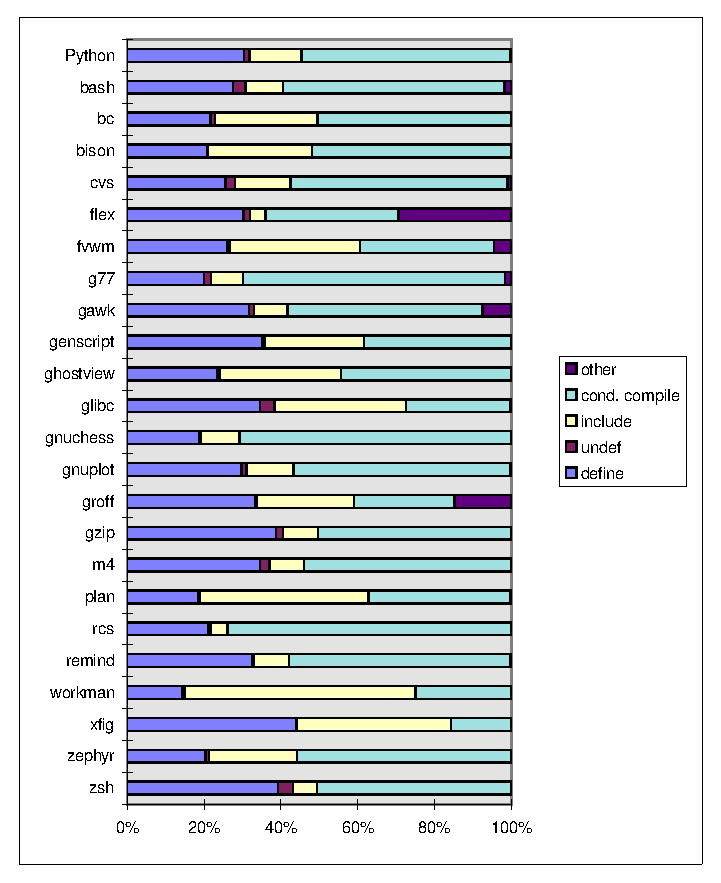
\epsfig{file=directives-breakdown.eps}}
\caption{Type of directive as a fraction of total directives.}
\label{fig:total_directives}
\end{figure}

\section{Frequency of Defined Macro Usage}
\label{sec:usage}

The second question we asked was: where and how often are macros
defined and used in practice?  

%Specifically, for each macro we
%determined:
%\begin{itemize}\itemsep 0pt \parskip 0pt
%
%\item How many times it was {\tt \#define}d.
%\item How many times it was {\tt \#undef}ed.
%\item How many arguments (if any) it takes.
%\item How many times (and where) it was mentioned in C source code.
%\item How many times (and where) it was mentioned in other
%preprocessor directives.
%
%\end{itemize}
%[FIX: gjb: This is redundant with the same information in paragraph
%form, above]

%[FIX: gjb: I'd also like to see info about how often define-d to the same
%expansion, or not, etc.]

\begin{figure}
{\small
  \setlength{\tabcolsep}{.25em}
  \begin{tabular}{|l|r|r|r|r|r|r|r|r|r|r|r|r|r|}\hline
\# Definitions & Python & bash & bc & bison & cvs & flex & fvwm & g77 & gawk & genscript & ghostview & glibc\\\hline\hline
1 & 71.86 & 21.52 & 53.25 & 63.21 & 34.60 & 41.10 & 55.21 & 83.45 & 40.37 & 75.19 & 50.35 & 19.46\\\hline
2 & 84.48 & 34.49 & 100.00 & 87.74 & 66.09 & 85.21 & 82.00 & 93.52 & 70.82 & 89.15 & 75.89 & 52.14\\\hline
3 & 89.93 & 39.85 & 100.00 & 87.74 & 78.31 & 87.47 & 89.24 & 95.83 & 79.82 & 89.15 & 90.78 & 68.57\\\hline
4 & 92.36 & 48.12 & 100.00 & 91.51 & 86.05 & 90.48 & 90.12 & 96.59 & 81.66 & 92.25 & 96.45 & 75.47\\\hline
5 & 94.18 & 51.88 & 100.00 & 91.51 & 87.78 & 94.24 & 90.67 & 96.83 & 82.24 & 92.25 & 100.00 & 79.95\\\hline
6 & 96.36 & 54.70 & 100.00 & 91.51 & 88.60 & 97.24 & 90.67 & 96.83 & 82.93 & 92.25 & 100.00 & 84.32\\\hline
7 & 96.79 & 55.69 & 100.00 & 91.51 & 89.57 & 97.24 & 92.97 & 98.18 & 82.93 & 92.25 & 100.00 & 86.58\\\hline
8 & 97.76 & 56.44 & 100.00 & 91.51 & 90.12 & 97.24 & 93.85 & 98.94 & 83.85 & 92.25 & 100.00 & 90.28\\\hline
9 & 98.30 & 57.28 & 100.00 & 100.00 & 90.12 & 97.24 & 94.84 & 98.94 & 85.93 & 92.25 & 100.00 & 91.16\\\hline
10+ & 100.00 & 100.00 & 100.00 & 100.00 & 100.00 & 100.00 & 100.00 & 100.00 & 100.00 & 100.00 & 100.00 & 100.00\\\hline
\multicolumn{12}{c}{} \\
\hline
\# Definitions & gnuchess & gnuplot & groff & gzip & m4 & plan & rcs & remind & workman & xfig & zephyr & zsh\\\hline\hline
1 & 67.10 & 69.76 & 33.06 & 35.48 & 32.82 & 72.55 & 56.83 & 35.61 & 68.33 & 86.69 & 61.31 & 78.79\\\hline
2 & 78.06 & 82.35 & 75.86 & 70.40 & 72.36 & 96.08 & 83.06 & 38.87 & 91.67 & 91.72 & 88.82 & 94.64\\\hline
3 & 89.68 & 86.38 & 85.14 & 79.78 & 75.24 & 98.43 & 91.26 & 42.45 & 91.67 & 93.61 & 92.67 & 96.39\\\hline
4 & 96.13 & 90.51 & 92.27 & 86.40 & 87.52 & 100.00 & 95.63 & 45.49 & 91.67 & 94.03 & 94.22 & 97.32\\\hline
5 & 96.13 & 92.57 & 92.27 & 90.99 & 88.48 & 100.00 & 95.63 & 46.58 & 100.00 & 95.60 & 94.86 & 97.32\\\hline
6 & 100.00 & 93.81 & 98.69 & 94.30 & 89.64 & 100.00 & 95.63 & 46.58 & 100.00 & 96.23 & 95.63 & 97.32\\\hline
7 & 100.00 & 94.53 & 98.69 & 98.16 & 89.64 & 100.00 & 95.63 & 49.62 & 100.00 & 96.23 & 95.63 & 97.32\\\hline
8 & 100.00 & 95.36 & 98.69 & 98.16 & 89.64 & 100.00 & 100.00 & 49.62 & 100.00 & 96.23 & 96.66 & 97.32\\\hline
9 & 100.00 & 95.36 & 98.69 & 98.16 & 91.36 & 100.00 & 100.00 & 50.60 & 100.00 & 96.23 & 96.66 & 97.32\\\hline
10+ & 100.00 & 100.00 & 100.00 & 100.00 & 100.00 & 100.00 & 100.00 & 100.00 & 100.00 & 100.00 & 100.00 & 100.00\\\hline
\end{tabular}
% Local Variables: 
% mode: latex
% TeX-master: "paper"
% End: 
%
}
\caption{Number of definitions per Cpp identifier.  The numbers in the
  table represent the percentage of identifiers which are defined a given
  number of times or fewer.  For example, bison contains 4 or fewer
  definitions for 91.51\% of all Cpp macros it defines, and no
  macro is defined 5, 6, 7, 8, or more than 9 times.}
\label{fig:define_count}
\end{figure}

Figure~\ref{fig:define_count} shows a histogram with cumulative
percentages of the number of times each identifier is {\tt define}d
in each of the packages.  The leftmost column lists the number of
times an identifier is {\tt define}d, with the one through nine counts
listed explicitly and all counts ten or greater collapsed into a
single bin.  
For example, in the python package, 94.18\% of
the identifiers were {\tt \#define}d five or fewer times.  

Going out to five or fewer separate {\tt \#define}s per symbol covers
over 90\% of the symbols for all but four packages: CVS is nearly
90\%, gawk and glib are about 80\%, and remind is under 50\%.  One
factor in the gawk and glib packages is that they are both highly
portable and also quite dependent on system libraries.  Remind uses macro
definitions to provide localization support for ten different natural
languages (and multiple character sets for some of them), accounting for
the surprisingly large number of macros with many definitions.  The
cumulative percentage rises to nearly 100\% at 12 definitions per symbol
for remind.

That there is a fairly limited use of multiple definitions of symbols
allows us to more reasonably bound the analysis needed to determine
the interactions among the definitions for a given symbol.

\begin{figure}
{\small
  \setlength{\tabcolsep}{.25em}
  \begin{tabular}{|l|c|c|c|c|c|c|c|c|c|c|c|c|c|}\hline
\#Uses & bc & bison & cvs & fvwm & genscript & gnuchess & gnuplot & gzip & plan & remind & workman & xfig & zsh\\\hline\hline
0 & 6.78 & 6.10 & 7.44 & 6.53 & 1.85 & 4.51 & 39.64 & 10.12 & 4.13 & 4.66 & 0.00 & 4.05 & 2.26\\\hline
1 & 18.64 & 14.63 & 24.97 & 33.28 & 20.37 & 25.82 & 56.61 & 33.13 & 23.39 & 32.84 & 34.69 & 44.44 & 18.73\\\hline
2 & 37.29 & 30.49 & 42.38 & 49.85 & 39.81 & 41.80 & 70.60 & 52.45 & 47.71 & 53.19 & 55.10 & 58.45 & 38.38\\\hline
3 & 47.46 & 53.66 & 51.38 & 57.75 & 53.70 & 51.64 & 79.02 & 65.64 & 56.88 & 61.03 & 63.27 & 66.32 & 49.93\\\hline
4 & 57.63 & 65.85 & 59.06 & 66.72 & 60.19 & 59.02 & 83.42 & 73.31 & 61.47 & 69.85 & 65.31 & 71.41 & 58.43\\\hline
5 & 69.49 & 73.17 & 66.03 & 71.43 & 66.67 & 63.11 & 87.31 & 78.83 & 65.60 & 75.25 & 71.43 & 73.84 & 65.21\\\hline
6 & 71.19 & 76.83 & 69.75 & 76.44 & 73.15 & 65.98 & 90.03 & 81.60 & 76.15 & 79.90 & 73.47 & 77.31 & 70.52\\\hline
8 & 74.58 & 79.27 & 75.15 & 80.24 & 75.93 & 72.13 & 91.84 & 88.65 & 82.57 & 83.33 & 77.55 & 82.18 & 78.49\\\hline
10 & 77.97 & 82.93 & 79.83 & 84.04 & 80.56 & 77.46 & 93.26 & 92.02 & 87.16 & 86.76 & 81.63 & 86.81 & 83.13\\\hline
20 & 84.75 & 95.12 & 90.16 & 93.77 & 88.89 & 86.07 & 95.85 & 96.93 & 93.58 & 93.63 & 87.76 & 93.17 & 91.50\\\hline
40 & 89.83 & 96.34 & 95.44 & 97.26 & 95.37 & 91.80 & 97.28 & 98.47 & 98.17 & 95.83 & 93.88 & 96.88 & 97.74\\\hline
80 & 98.31 & 97.56 & 97.48 & 98.63 & 98.15 & 95.90 & 98.58 & 99.39 & 98.62 & 97.79 & 95.92 & 98.73 & 99.47\\\hline
$>$80 & 100.00 & 100.00 & 100.00 & 100.00 & 100.00 & 100.00 & 100.00 & 100.00 & 100.00 & 100.00 & 100.00 & 100.00 & 100.00\\\hline
%\hline
\end{tabular}
% Local Variables: 
% mode: latex
% TeX-master: "paper"
% End: 
%
}
\caption{Number of expansions per Cpp macro.  The numbers in the
  table represent the percentage of identifiers which are expanded a given
  number of times or fewer.  For example, fvwm expands 49.85\% of its
  macros two or fewer times.}
\label{fig:use_count}
\end{figure}

Figure~\ref{fig:use_count} is structured as the previous figure, but it
represents the number of times that a defined name is expanded in
either C code or preprocessor directives.  For instance, in the bc
package, 74.58\% of the macros were expanded eight or fewer times.

It is notable that most packages contain a significant number of defined
macros that are never expanded.  (Figure~\ref{fig:use_count} reports only
on macros defined in a package, not those defined in system or library
header files, inclusion of which pushes the unused percentage well above 50\%.)
Most packages are in the 3-10\% range, while gnuplot
reaches nearly 40\%.  Although it's difficult to fully account for the
larger numbers, contributing factors include a lot of cut-and-paste
and a lack of attention to implementations for specific platforms in
some packages.  Again with respect to bounding analysis, covering
macros with 10 or fewer uses covers approximately 75-80\% of the cases.

\begin{figure}
\centerline{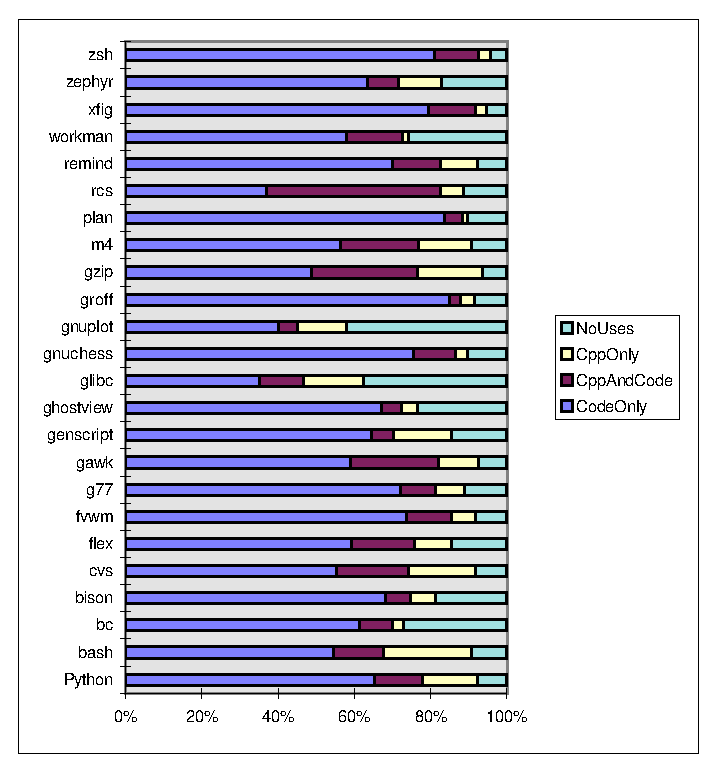
\epsfig{file=usage.eps}}
%{\small
%  \setlength{\tabcolsep}{.25em}
%  \begin{tabular}{|l|r|r|r|r|}\hline
Package & CodeOnly & CppAndCode & CppOnly & NoUses\\\hline
Python & 861 & 166 & 193 & 100\\\hline
bash & 348 & 84 & 147 & 59\\\hline
bc & 43 & 6 & 2 & 19\\\hline
bison & 62 & 6 & 6 & 17\\\hline
cvs & 401 & 137 & 128 & 59\\\hline
flex & 162 & 46 & 26 & 40\\\hline
fvwm & 489 & 77 & 42 & 55\\\hline
gawk & 265 & 103 & 48 & 33\\\hline
genscript & 76 & 7 & 18 & 17\\\hline
gnuchess & 190 & 28 & 8 & 26\\\hline
gnuplot & 303 & 39 & 97 & 319\\\hline
groff & 420 & 14 & 18 & 42\\\hline
gzip & 144 & 82 & 50 & 19\\\hline
m4 & 122 & 44 & 30 & 20\\\hline
plan & 194 & 11 & 3 & 24\\\hline
rcs & 55 & 68 & 9 & 17\\\hline
remind & 293 & 52 & 41 & 32\\\hline
workman & 36 & 9 & 1 & 16\\\hline
xfig & 678 & 105 & 25 & 45\\\hline
zephyr & 354 & 46 & 63 & 96\\\hline
zsh & 590 & 84 & 24 & 31\\\hline
\end{tabular}
%
%}
\caption{Where Macro Uses Occur}
\label{fig:define_usage}
\end{figure}

Figure~\ref{fig:define_usage} shows the percentage of defined macros
that are used in C code, in Cpp code, in both, or in neither (i.e. no
uses).  No package expanded all of its defined macros; two did not
expand as many as 40\% of the defined macros.  The dominant usage was
in C code only; these uses don't, therefore, have any affect on
conditional compilation (for example).  


\section{Categorization}
\label{sec:categorization}

The third question we asked was: in what ways are the macros used in
practice?  In contrast to the earlier analyses, this requires an
analysis and categorization of the bodies of the macros to determine
how they can be used.  This analysis depends in part on some
heuristics we defined to interpret the bodies of the macros; by
studying our analyses, we have refined (and continue to refine) the
heuristics to do a better job of categorization.  A straightforward
refinement that we are pursuing looks at the specific uses of macros
to help in this categorization.

In addition to classifying each macro as taking arguments or not, our tool
identifies the following specific categories (and a few more rarely-used
ones omitted for reasons of space):
\begin{description}
  \sloppy
  \emergencystretch=2em

\item[Null define]  The {\tt \#define} gives only an
identifier name.  Such macros appear most frequently in Cpp directives
(such as {\tt \#ifdef}), but may also appear in code.  For instance,
macro {\tt private} may expand either to {\tt static} or to nothing,
depending on whether a debugging mode is set, or macro {\tt then} might
expand to nothing for programmers who like {\tt else} to be offset by
{\tt then}.\footnote{Recall that we are empirically studying the way
in which macros are used rather than assessing the desirability of any
particular usage style.}  Macros with null definitions are often used as boolean
variables by the preprocessor.

\item[Literal] The macro is defined to be a specific constant value;
  for instance, {\tt \#define NULL 0} or 
  {\tt \#define ETCHOSTS "/etc/hosts"}.  Such macros act like {\tt const}
  variables, albeit 
  without type information, debugging information in the symbol table,
  and so forth.  Macros with constant expression bodies, such as
  \verb|#define| \verb|RE_DUP_MAX| \verb|((1<<15)-1)|, are included, but
  not macros referencing other literal or constant macros, so this number
  underestimates the number of macros with constant values.

\item[Expression]  The macro body is an expression.  This expression
  might have a single constant value everywhere (the usual case for
  expression macros without arguments), or might have a different value on
  each use (the usual case for expression macros with arguments).  Of
  expression macros, 6.31\% use assignment operators,
  which have potentially unexpected results.  A macro argument that is
  assigned to is like a pass-by-reference function argument and need only
  be noted in the macro's documentation.  A global variable that is
  assigned to also presents no difficulties in understanding.  Assignment
  to a local variable, however, demands that such a variable exist wherever
  the macro is invoked, and assigns to different variables at different
  invocations.\footnote{By contrast, LCLint considers assignment to a macro
  argument dangerous but does not appear to check for assignments to local
  variables.}

%    * expression sans assignment
%    * expression with assignment

\item[Statement]  The macro body is a statement.  Such macros can be
  confusing to use, because programmers are inclined to add a semicolon
  after a call to such a macro, which can cause problems such as 
  mis-parsing of nested {\tt if} statements.  The
  well-known \verb|do {|\ldots\verb|} while (0)| partial statement trick
  solves this problem.  To our surprise, we found very few uses of that
  construct, but many instances of a macro that expanded to a statement
  like \verb|{|\ldots\verb|}| in which a call to the macro was immediately
  followed by a semicolon.

\item[Stringization and pasting]  The macro body contains {\tt \#} or
  {\tt \#\#}, which treat the macro argument not as a token but as a
  string.  No existing language mechanism can replace such macros.  Our
  implementation separates these categories, but we combine them to
  simplify our figures.

\item[Other syntactic macros]  Like stringization and pasting, these
  macros make essential use of the unique features of the preprocessor.
  Our framework separately categorizes a number of such macros, including
  those that expand to a reserved word (such as {\tt \#define private
  static}, mentioned above), those which expand to a delimiter such as
  {\tt ,} or {\tt ;}, and those with mismatched parentheses, brackets, or
  braces.  (The latter are often used to create a block and perform actions
  that must occur at its beginning and end, such as \verb|BEGIN_GCPRO| and
  \verb|END_GCPRO|.)

\item[Classification failure]  Frequent reasons that our
classification heuristics failed
  include multiple adjacent identifiers
  ({\tt \#define EXFUN(name, proto) name proto},
  {\tt \#define \verb|DO_OP|(OP,a,b) (a OP b)}) and illegal identifier
  names ({\tt \#define \verb|FAT$C_VFC| 3} for VMS compilation), tokens %$HACK
  ({\tt \#define \verb|LIB_PATH| /usr/ucblib}), and constants ({\tt 1ULL} for
  {\tt unsigned long long}).  Of the fewer than 1000 classification
  failures in the 24 packages, over half appeared in gnuplot; gnuplot, cvs,
  and groff accounted for over 75\% of the failures, many of which could be
  eliminated by slightly relaxing the parsing rules.  Only five packages had no
  macro classification failures at all.


% \item {\em Constants\/}, where the {\tt \#define} gives only an
% identifier name and a value.
% 
% \item {\em Null defines\/}, where the {\tt \#define} gives only an
% identifier name.
% 
% \item {\em Functions\/}, where the {\tt \#define} has one or more
% parameters.  The functions are broken down into several sub-categories:
% \begin{itemize}
% 
% \item {\em Functions/Cpp\/}, where the body of the macro invokes one
% or more other macros.  [FIX: This is currently ``function, macro as
% function'', I think.]
% 
% \item {\em Functions/C-expression\/}, where the body of the macro is
% defined as a well-defined C expression.  [FIX: This is currently
% ``function, some constant'', I think.]
% 
% \item {\em Functions/Essential\/}, [FIX: bad name?] where the body of the
% macro is not defined as a C expression; specific reasons include
% ...
% 
% These are of special interest with respect to translation.  Some of
% them, for instance ones that define C statements rather than
% expressions, might yield to translation if further analysis shows that
% they are used in particular, disciplined ways.
% 
% \end{itemize}
% 
% \item{\em Uncategorized\/}, where we could not characterize the macro
% as any of the above categories.

\end{description}

Figure~\ref{fig:categorization} shows the percentage of macros that
fit into these categories for each package.  The null define and
literal categories together account for nearly 60\% of all
macro definitions; converting these into C++ constructs
should be simple.  The extremely small percentage (0.33\%) of
``essential'' macros---those such as stringization and pasting that
have no simple mapping into any programming language---is encouraging;
these would have to be studied individually, but the overall cost
may well be low.  Further analysis of the conditional compilation
structure (in the style of Krone and Snelting~\cite{Krone94}) and of
the macros with free variables (essentially achieving dynamic scoping)
is needed to see which of the roughly 33\% of expression macros should
be easy to handle in a conversion process.

\begin{figure}
{\small
  \setlength{\tabcolsep}{.25em}
  \begin{tabular}{|l|c|c|c|c|c|c|c|}\hline
Package & Null define & Literal & Expression & Statement & Stringization and pasting & Other syntatic macros & Failed classification\\\hline
Python & 176 & 510 & 865 & 50 & 5 & 62 & 21\\\hline
bash & 717 & 679 & 637 & 3 & 3 & 62 & 30\\\hline
bc & 4 & 36 & 37 & 2 & 0 & 9 & 1\\\hline
bison & 4 & 64 & 32 & 0 & 0 & 2 & 0\\\hline
cvs & 106 & 683 & 530 & 58 & 0 & 69 & 116\\\hline
flex & 32 & 224 & 87 & 19 & 0 & 36 & 2\\\hline
fvwm & 48 & 748 & 122 & 11 & 0 & 27 & 1\\\hline
gawk & 49 & 243 & 391 & 11 & 0 & 59 & 23\\\hline
genscript & 8 & 71 & 39 & 0 & 0 & 9 & 0\\\hline
gnuchess & 12 & 201 & 93 & 5 & 0 & 5 & 1\\\hline
gnuplot & 134 & 577 & 244 & 3 & 0 & 18 & 9\\\hline
groff & 18 & 607 & 148 & 11 & 1 & 36 & 98\\\hline
gzip & 110 & 229 & 130 & 25 & 0 & 21 & 4\\\hline
m4 & 36 & 83 & 272 & 26 & 0 & 62 & 1\\\hline
plan & 9 & 208 & 43 & 4 & 0 & 4 & 2\\\hline
rcs & 15 & 54 & 80 & 14 & 0 & 18 & 3\\\hline
remind & 11 & 744 & 108 & 65 & 0 & 18 & 2\\\hline
workman & 1 & 41 & 25 & 2 & 0 & 0 & 0\\\hline
xfig & 31 & 681 & 240 & 24 & 0 & 20 & 0\\\hline
zephyr & 80 & 451 & 255 & 28 & 0 & 27 & 2\\\hline
zsh & 31 & 520 & 267 & 20 & 0 & 40 & 5\\\hline
\hline
Total & 1632 & 7654 & 4645 & 381 & 9 & 604 & 321\\\hline
\end{tabular}%
}
\caption{Categorization of macro definition bodies; each row sums to 100\%.}
\label{fig:categorization}
\end{figure}





%In anticipation of the translator tool, the analysis tool infers
%types, using techniques similar to those of Siff and Reps~\cite{Siff-fse96}
%and O'Callahan and Jackson~\cite{OCallahan-icse97}.  Our use of the
%type information is in the early stages, however, and we do not report
%on the preliminary results in this paper.

% [FIX: Benefits even from simple literal constant conversion -- exposes
% symbolic information to the debugger]

%[FIX: Should this also include Mike's manual breakdown into categories
%for gzip.  --not tonight!]

\section{Conclusion}
\label{sec:discussion}

Even with significant expertise in using C, C++, and the Cpp macro
preprocessor, these data showed us a far broader and diverse use of
preprocessing than we had anticipated.  

We wrote a collection of Perl scripts to produce and analyze these
data.  As we developed them, we slowly shifted from a lexical analysis
of the source to a syntactic analysis of the source.  For example, we
now properly parse virtually all declarations in every package.  We're
pursuing even more analysis, pushing into semantics.  For instance, we
can now determine which identifiers are free variables within a
defined macro.  We are also close to inferring the types of
macro bodies, one of several steps necessary before we
can attempt to build a converter from C to C++.  Once we can usefully
convert C to C++, eliminating most macro usages (except for
{\tt \#include}s), this would not only programmers to shift to C++ and
its constructs more easily, but even more importantly, it would
greatly simplify the development of source-level debuggers, call graph
extractors, and other programming support tools.

%[FIX: We catch errors that you miss when you look at post-processed code
%since we look at all branches.]
%
%[FIX: Harsh macro examples?]

% Not really right:  Don't want the ``References'' section head to be small.
{\small \bibliography{evil}}

\end{document}
